\documentclass[twocolumn]{ctexart}
% ctexart、ctexrep、ctexbook和ctexbeamer, 对应 LaTeX 的article、report、book和beamer
\usepackage[a4paper,left=3cm,right=3cm,top=2.6cm,bottom=2.6cm]{geometry} % 设置页面尺寸
\usepackage{fancyhdr} % 设置页眉页边页脚
\usepackage{multicol} % 多栏排版
\usepackage{xeCJK} % 中文支持
\usepackage{ctex} % 中文支持
\usepackage{footmisc} % 控制脚注格式,包括编号、字体、分隔线等
\usepackage{titletoc} % 定制目录列表样式
\usepackage{fontspec} % XeTeX下的字体选择宏包
\usepackage{setspace} % 行距
\usepackage{graphicx} % 插图
\usepackage{pdfpages} % 引用pdf页面
\usepackage{booktabs} % 三线表
\usepackage{multirow} % 表格多行支持
\usepackage{caption} % figure和table等中的说明文字
\usepackage{tikz} % 绘图
\usepackage{etoolbox} % 给宏包打补丁
\usepackage{hyperref} % 超链接
\usepackage{xcolor} % 颜色支持
\usepackage{array} % 数学表格
\usepackage{amsmath} % 数学公式
\usepackage{amssymb} % 数学字体与符号
\usepackage{amsthm} % 数学定理格式
\usepackage{subfig} % 排版子图
\usepackage{float} % 浮动体格式控制
\usepackage{lmodern} % 一种字体支持
\usepackage{listings} % 插入代码
\usepackage{tcolorbox} % 好看的块环境
\usepackage{pifont} % 字体支持
\usepackage{perpage} %the perpage package
\usepackage{mathdesign} % some math fonts
\usepackage{ulem} %一些文字强调的宏包
\usepackage{fancyvrb} % some fancy verbatim 
\usepackage{enumitem} % 列表项目
\usepackage{txfonts} % 一些字体
\usepackage{makecell}
\usepackage{mathrsfs}
\usepackage{subfig}                 % 子图包,不要与{subfigure}混用,{subfig}较新
\usepackage{overpic}   
%重置每页脚注序号
\pagestyle{headings}
\MakePerPage{footnote} %the perpage package command
\renewcommand \thefootnote{\ding{\numexpr171+\value{footnote}}}
% 为tcolorbox导入三个程序包
\tcbuselibrary{skins, breakable, theorems} 

% 设置代码格式 - 关键字加粗, 其余为正常。非彩色
\lstset{
    aboveskip=5mm,
    belowskip=5mm,
    breaklines=true,
    breakatwhitespace=true,
    columns=flexible,
    extendedchars=false,
    showstringspaces=false,
    numbers=none,
    basicstyle={\small\ttfamily},
    captionpos=t,
    frame=tb,
    tabsize=4
}

\lstdefinestyle{cpp} {
  language=C++
}

\lstdefinestyle{c++} {
  language=C++
}

\lstdefinestyle{python} {
  language=python,
  morekeywords={as}
}


% 为目录添加 PDF 链接
\addtocontents{toc}{\protect\hypersetup{hidelinks}}

% 设置「目录」二字格式
\renewcommand{\contentsname}{
  \fontsize{16pt}{\baselineskip}
  \normalfont\heiti{目~~~~录}
  \vspace{-8pt}
}

% 定理、定义、证明
\newtheorem{theorem}{定理}[section]
\newtheorem{definition}{定义}[section]
\newtheorem{lemma}{引理}[section]
\newtheorem{corollary}{推论}[section]
\newtheorem{example}{例}
\newtheorem{proposition}{命题}[section]

\title{模电作业}
\author{2021251124 古翱翔}
\date{\today}

\begin{document}

% 显示标题作者时间
\maketitle
\newpage

% 调整目录行间距
\renewcommand{\baselinestretch}{1.35}
% 添加目录
\tableofcontents
\newpage

% 正文 22 磅的行距
\setlength{\parskip}{0em}
\renewcommand{\baselinestretch}{1.53}

% \section{序}
% 从电子管(1904)到晶体管(1947),再到集成电路(1958),再到超规模集成电路(1980)。摩尔定律,18-24。
% \section{半导体器件}
P3N5(3p)(穴电),PN结多子扩散形成电流,
\subsection{二极管}
\begin{figure}[H]
    \centering
    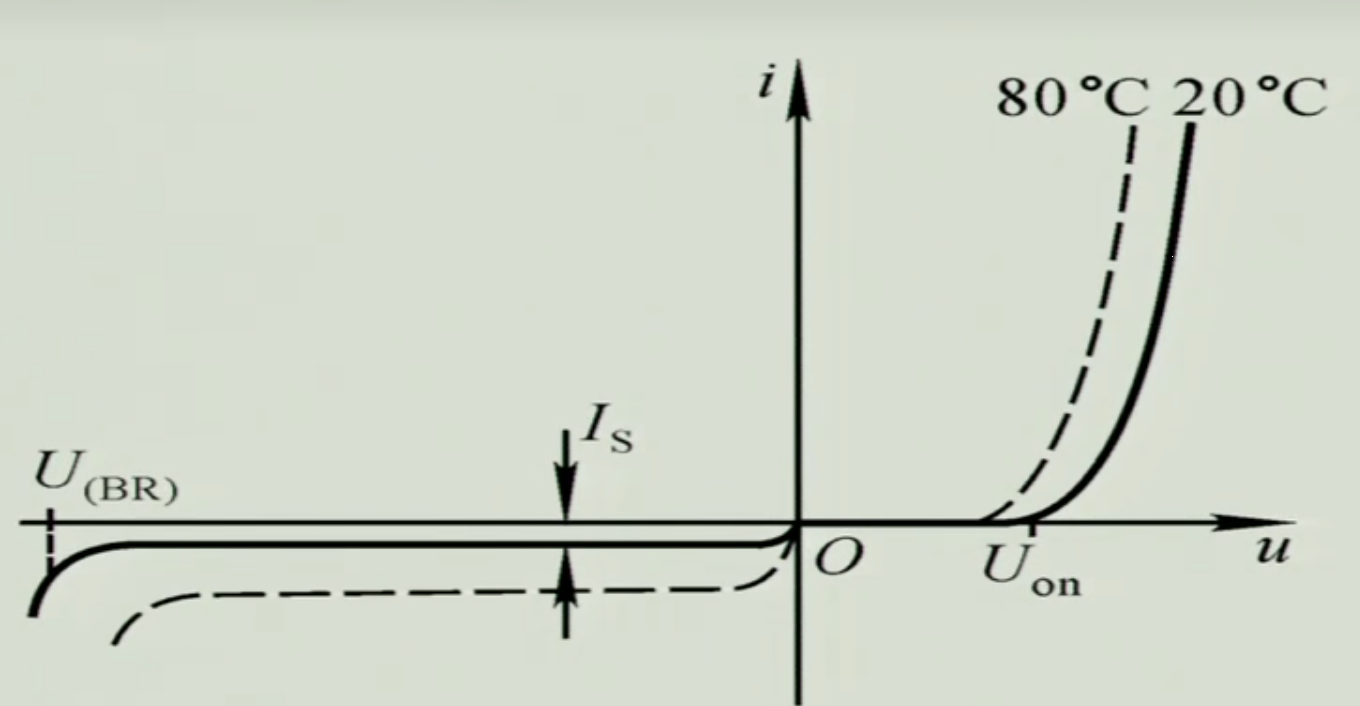
\includegraphics[width=7cm]{./img/1.2.png}
\end{figure}
击穿电压:$U_{BR}$,开启电压:$U_{on}$,反向电流:$I_s$,最高频率$f_m$。温度升高,左下。
\subsubsection{等效电路}
我们需要知道等效电路是什么样子的,用非线性用线性表示出来。有两种,一种是外特性的等效,一种是模型原理上的等效。伏安特性折线化
\begin{theorem}[二极管电流方程]
\[
i=I_s(e^{\frac{u}{U_T}}-1)
\]
\end{theorem}

可以等效成理想,考虑压降,考虑压降和线性斜率,微变等效电路。

对于微变等效电路,已正向导通,有
\begin{equation}
I=I_se^{\frac{U}{U_T}}    \tag{2.1}
\end{equation}
\subsubsection{怎么计算工作状态}
\begin{description}[leftmargin=1.7cm,style=nextline,nosep]% nosep没有垂直间隔
    \item[只有一个] 断开算两端电压
    \item[两个或者多个] 共阴阳只有一个可以正常工作,可以看谁不共的大或者使用\underline{\textbf{假设}}法。
    \item[稳压二极管] 工作在击穿区?
    \item[其他] SI 0.7, GE 0.2    
\end{description}
\subsection{双极型晶体管}
\subsubsection{晶体管的主要参数}
极限参数有最大允许功耗,集电极最大允许电流$I_CM$,反向击穿电压$U_{(BR)CEO}$
% \subsubsection{三极管的h参数等效电路}
% 在交流通路中可将晶体管看成为一个二端口网络,输入回路、输出回路各为一个端口

\subsection{单极型晶体管FET}
低功耗,噪声小,体积小,抗辐照性强,只有\textbf{\underline{多子}}参与导电,\underline{\textbf{压控}}。
分为\underline{结}型(JET)和\underline{绝缘栅}型(MOS管)。
\subsubsection{N沟道增强型绝缘栅型MOS管}
        \begin{figure}[H]
            \centering
            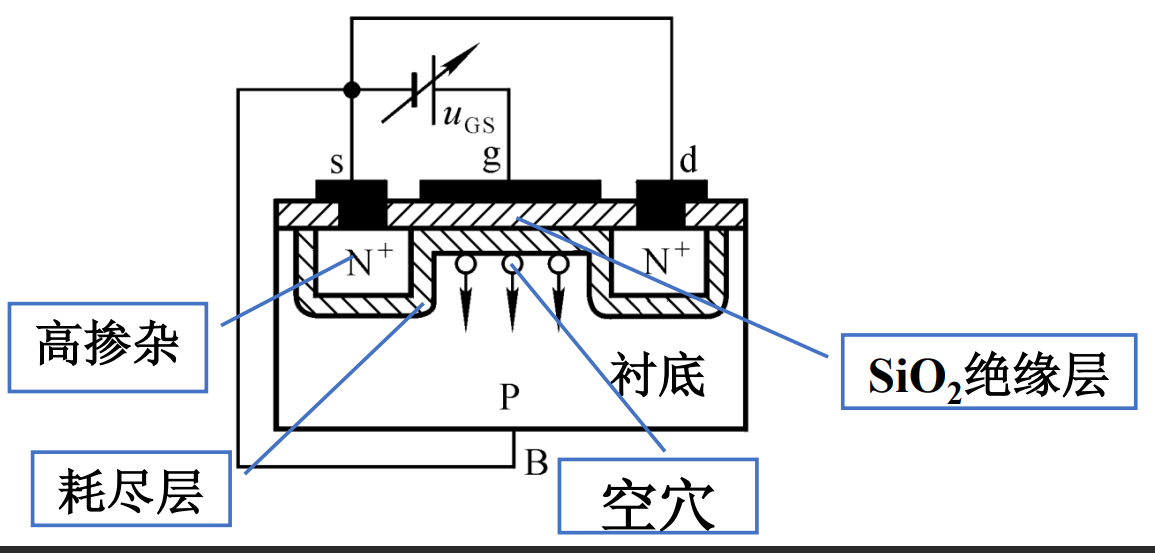
\includegraphics[width=7cm]{img/1.3.png}
            \end{figure}
g 栅极,S 源极,d漏极,分别对应三极管的(b,e,c),$U_{GS}$ 增大到一定程度,再继续增大,
导电沟道将变厚,ds之间\underline{\textbf{电阻}}变小。
        \begin{figure}[H]
            \centering
            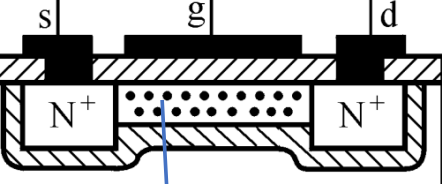
\includegraphics[width=5cm]{img/1.4.png}
            \end{figure}
此时如果要出现电流,那我们只需要在ds两端加一个电压$U_{ds}$就行,此时固定USG,研究$U_{ds}$对$i_D$的影响,gs电位差变小,沟道开始
倾斜,$U_{ds}$增大,沟道越来越倾斜,$i_D$增大,但是增大的速度越来越慢,最后趋于饱和。
        \begin{figure}[H]
            \centering
            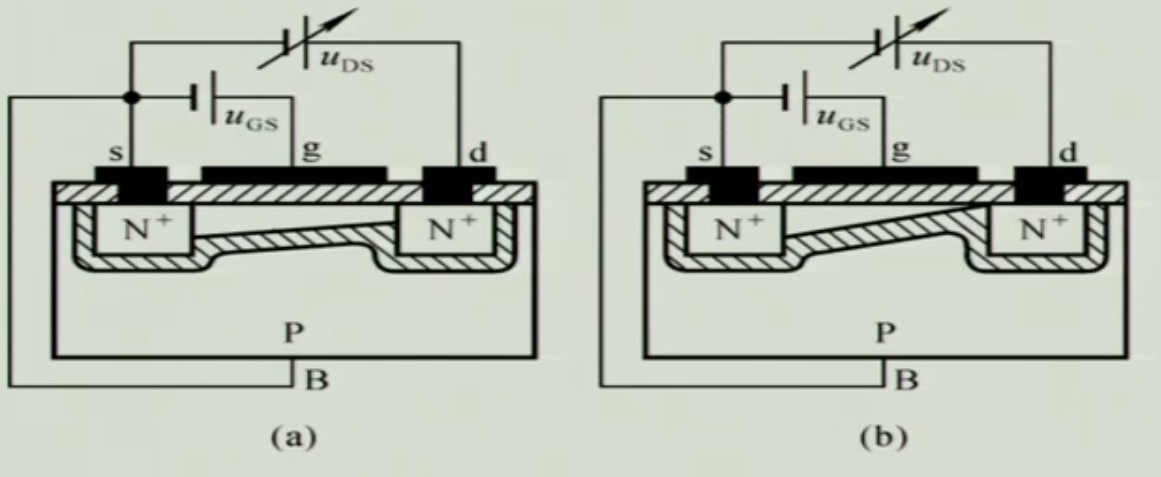
\includegraphics[width=7cm]{img/1.5.png}
            \end{figure}
当$\displaystyle U_{GS}-U_{DS}=U_{GS(th)}$ 成为预夹断,再增加电阻增大,之后近似恒流。
\begin{figure}[H]
    \centering
    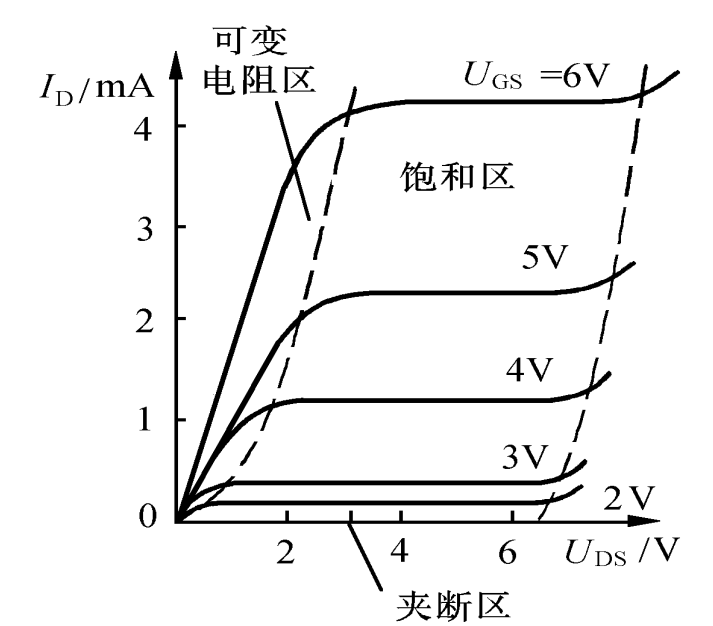
\includegraphics[width=7cm]{img/1.6.png}
    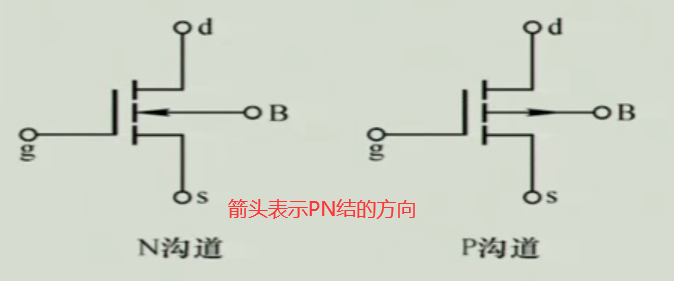
\includegraphics[width=7cm]{img/1.7.png}
    \end{figure}
他本身没有沟道,那能不能让他一开始就有沟道?
\begin{quote}
{\qquad\parindent2\ccwd\kaishu\zihao{5}
N 沟道耗尽型MOS管
}
\subsubsection{N沟道耗尽型绝缘栅型MOS管}
天生有沟道,有一个参数叫做$U_{GS(off)}$,称作夹断电压。
\end{quote}
\subsubsection{N沟道结型场效应管}
        \begin{figure}[H]
            \centering
            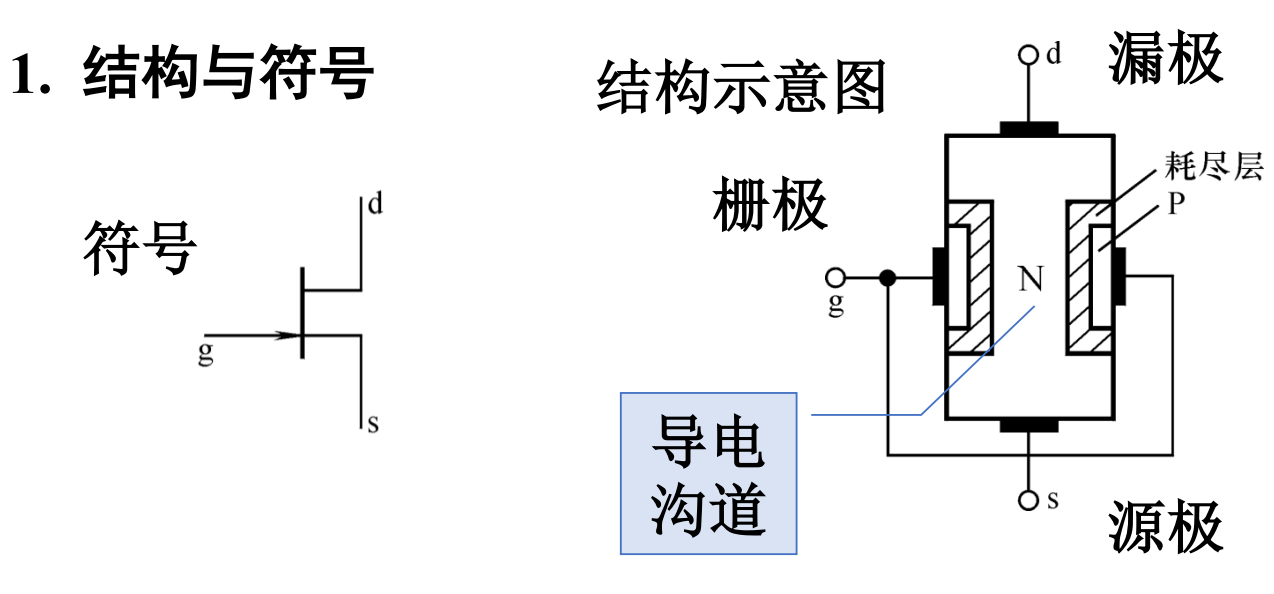
\includegraphics[width=7cm]{img/1.8.png}
            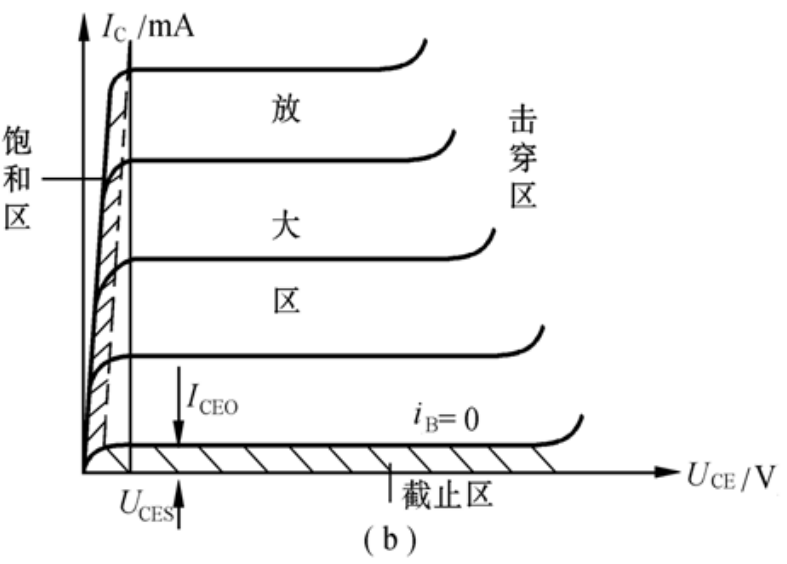
\includegraphics[width=7cm]{img/1.9.png}

            \end{figure}
天生有沟道,加反压使其夹断,是真夹断。

\subsection{场效应管的特性曲线和参数}
漏极,源极和栅极。有转移和输出特性曲线。
\begin{figure}[H]
    \centering
    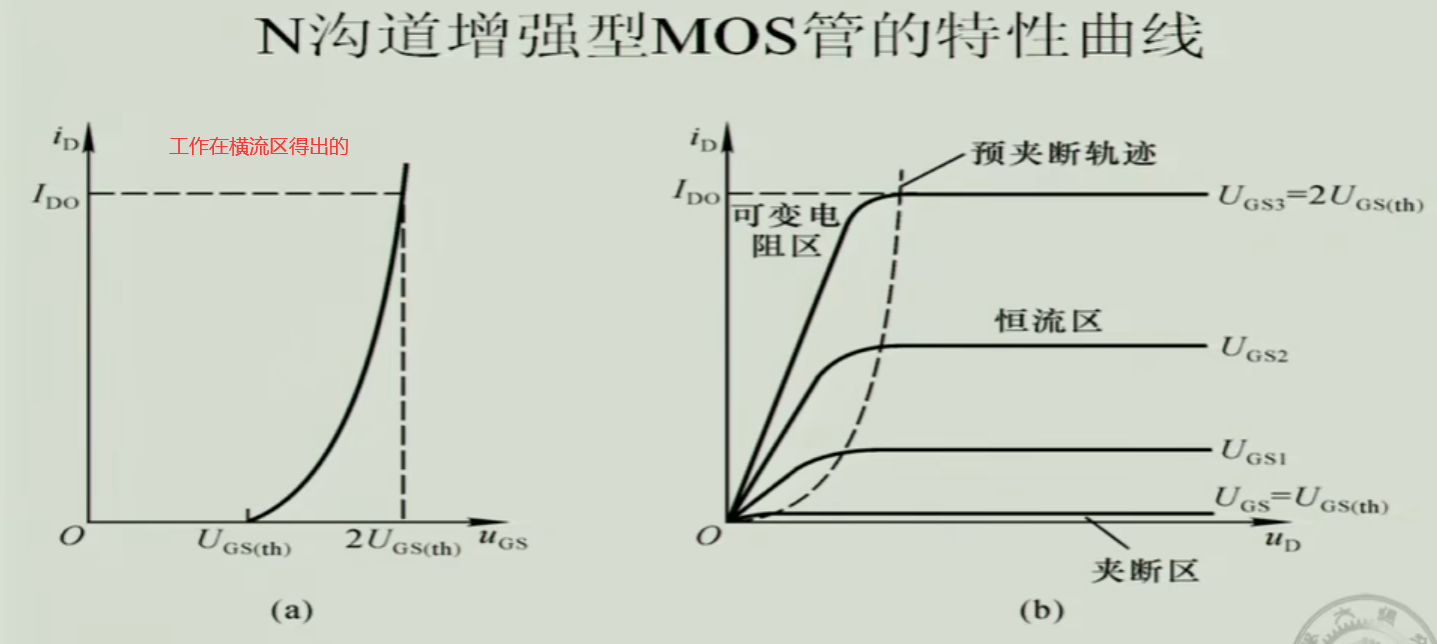
\includegraphics[width=7cm]{img/1.9.1.png}
    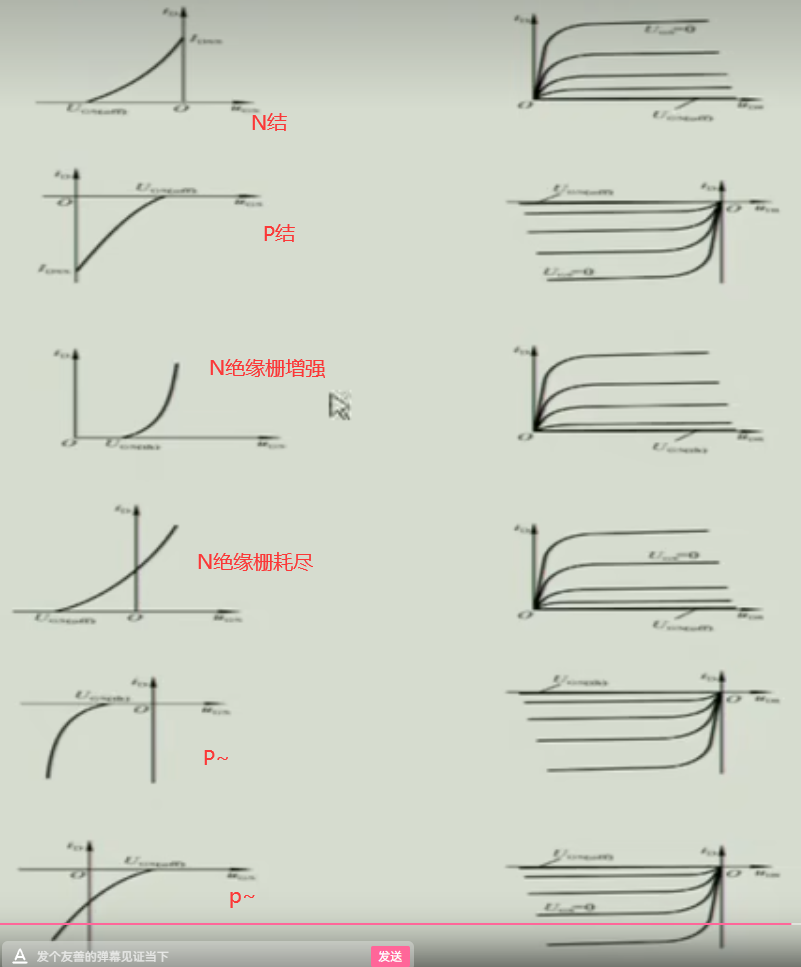
\includegraphics[width=8cm]{img/1.9.2.png}

    \end{figure}
其中漏极电流和gs之间电流方程为(对应上图曲线)
\begin{align}
    i_{D}=I_{DO}(\frac{u_{GS}}{U_{GS(th)}}-1)^{2} \tag{2.1.a} \\
    i_{D}=I_{DSS}(1-\frac{u_{GS}}{U_{GS(off)}})^{2} \tag{2.1.b}
\end{align}

其中$I_{Dss}$为$U_{GS}=0$ 时的漏极电流,
其中$I_{Do}$为$U_{GS}=2U_{GS(th)}$ 时的漏极电流.(2.1.a)是对N沟道绝缘栅型增强(MOS)管,(2.1.b)是对N沟道结型(JET)管。
{直流参数}
$$
U_{GS(th)},U_{GS(off)},I_{Dss},R_{GS(DC)}
$$
{交流参数}
跨导$g_m$
\section{基本放大电路}
        \begin{figure}[H]
            \centering
            
\includegraphics[width=7cm]{img/2.0.png}
            \end{figure}
是\underline{\textbf{功率}}放大,本质上还是能量控制和放大,必要条件是要有有源元件,前提是不失真,用\underline{\textbf{正弦波}}测试。

\subsection{怎样构建(基本放大电路)}
我们只有一个小功率信号,元件,电源。让晶体管工作在\underline{\textbf{放大}}区,小信号需要控制$i_B$,实际上是控制
$U_{BE}$。
        \begin{figure}[H]
            \centering
            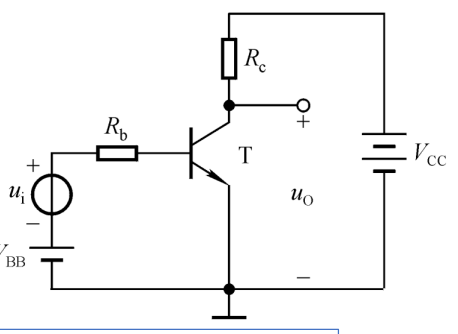
\includegraphics[width=7cm]{img/2.1.png}
            \end{figure}
首先是正反偏,然后输入加入电阻保护,加上输出电阻输出电压。
\begin{description}[leftmargin=0.9cm,style=nextline,nosep]% nosep没有垂直间隔
    \item[$V_{BB}$] 抬高小信号电压,使三极管发射结正偏。
    \item[$V_{\mathbb{C}}$] 使得三极管集电结反偏。
    \item[$R_b$] 保护。
    \item[$R_c$]  使得输出电压。
    \item[$u_i$] 输入电压     
    \item[静态工作点$Q$] $u_i=0$的时候,此时各个参数的表示为$I_{BQ},I_{CQ},U_{BEQ},U_{CEQ}$ 。
    \item[静态工作点的必要性] 因为要解决失真问题,使三极管工作在线性区,使信号不失真。  
\end{description}

% \subsubsection{共射放大电路}
对于共射放大电路,负载上无直流份量,也可以在输入或者输出加上\underline{\textbf{耦合电容}}来隔离\textbf{直流},通过交流,叫做阻容耦合电路。
% \subsection{分析方法}
我们按照过程(电容耦合下),有如下
\begin{align}
u_{BE}&=u_i \tag{3.1.a}\\
i_{B}&=\frac{u_{CC}-u_{BE}}{R_{B}} \tag{3.1.b}\\
i_{C}&=\beta i_{B} \tag{3.1.c}\\
u_{CE}+R_Ci_C&=u_{CC}    \tag{3.1.d}
\end{align}
\subsubsection{性能参数}
\begin{figure}[H]
    % \centering
    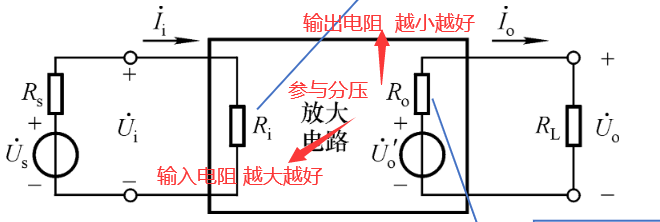
\includegraphics[width=7cm]{img/2.3.png}
    \end{figure}
    
任何一个放大电路都可以看作是一个二端口网路,定义放大倍数为输入和输出量之比,但是电压放大倍数$\dot{A_{uu}}$是最常被研究的
通频带
\begin{figure}[H]
        % \centering
        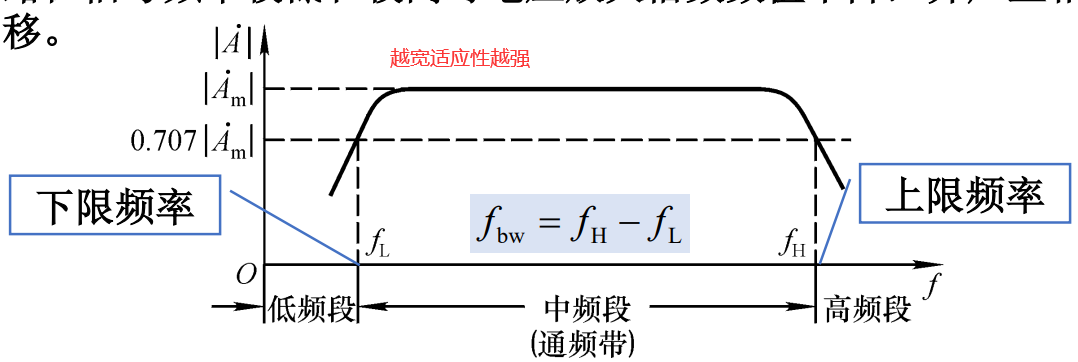
\includegraphics[width=7cm]{img/2.2.png}
        \end{figure}

\begin{definition}[非线性失真系数]
$$
D=\frac{\sqrt{\sum_{i=1}^{\infty}{U_{i+1}^2}}}{U_1}
$$
\end{definition}
最大输出功率$p_{om}$,电源效率为$\eta=\frac{p_{om}}{p_v}$
\subsubsection{直流通路和交流通路}
\begin{description}[leftmargin=1.7cm,style=nextline,nosep]% nosep没有垂直间隔
    \item[直流通路] $U_S=0$,电容开路,电感短路。用于研究静态工作点
    \item[交流通路] 直流电源短路,大容量电容短路。  用于动态参数研究
\end{description}

先静后动。静态有计算和图解,动态有图解和微变等效。
\subsection{静态分析方法}

\subsubsection{图解法}
在三极管的输入和输出曲线上,画出外部的工作线。
        \begin{figure}[H]
            \centering
            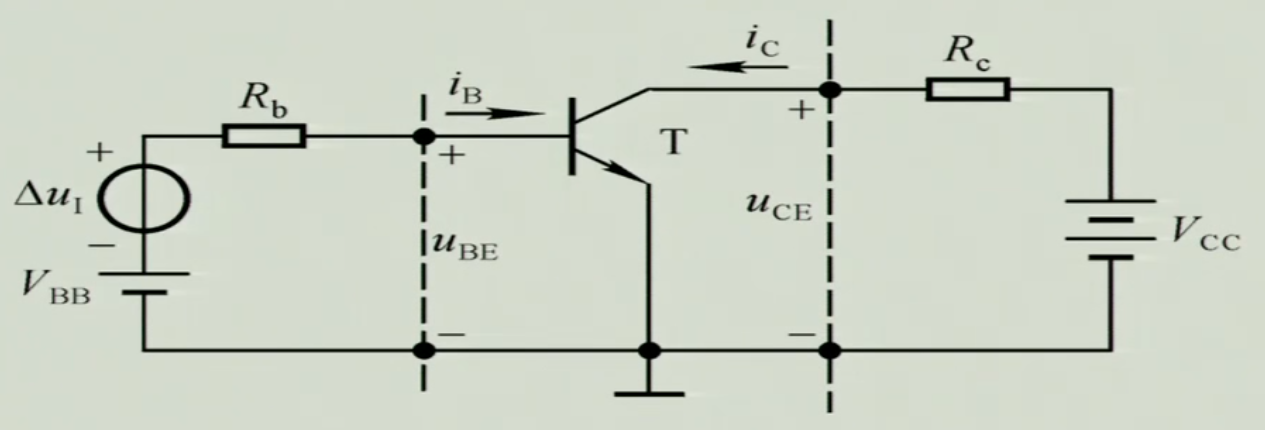
\includegraphics[width=7cm]{img/2.4.png}
            \end{figure}
\begin{align}
i_b=\frac{V_{BB}-U_{BE}}{R_b} \tag{3.1.a} \\
i_c=\frac{V_{CC}-U_{CE}}{R_c} \tag{3.1.b} 
\end{align}
(3.1.a)是对于输入曲线,(3.1.b)对于输出曲线。纵坐标是
$\displaystyle  \frac{V_{\mathbb{CC}}}{R_c}$,
横坐标是$V_{CC}$,对于放大倍数,有如下:
        \begin{figure}[H]
            \centering
            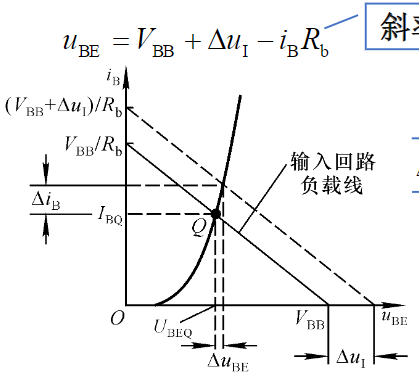
\includegraphics[width=7cm]{img/2.5.png}
            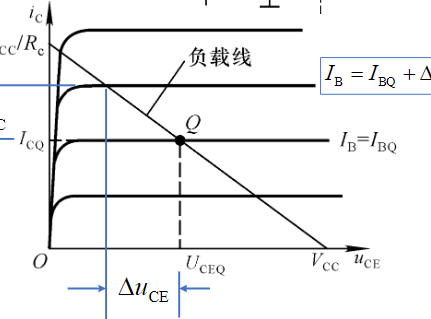
\includegraphics[width=7cm]{img/2.7.png}

            \end{figure}
\subsubsection{电位分析法}
一个一个地写起来,使用基尔霍夫电压定律。
\subsubsection{估算法}
本质是两个直线相交。利用$U_{BEQ=0.7V}$
        \begin{figure}[H]
            \centering
            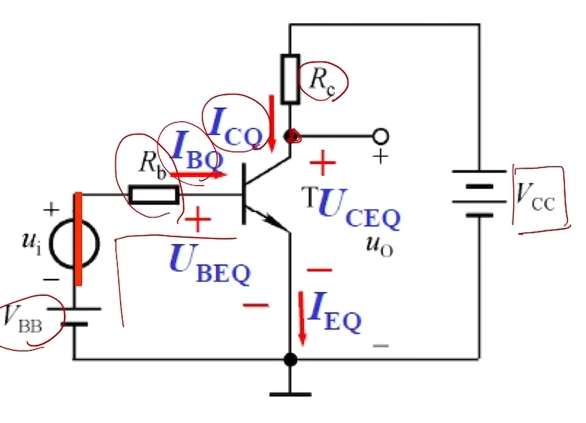
\includegraphics[width=7cm]{img/2.8.png}
            \end{figure}
\begin{align}
    V_{BB}=R_bI_{BQ}+0.7 \tag{3.2.a} \\
    I_{B_Q}:I_{CQ}:I_{EQ}=1:\beta:1+\beta\tag{3.2.b}
\end{align}

\subsubsection{等效电路}
先找Q点,再找$\displaystyle r_{be}=r_{bb}+(H\beta)\frac{U_T}{I_{EQ}}$

\subsubsection{静态分析法列写方程}

\subsection{动态分析}
\subsection{h参数等效电路}
中低频,小信号。
\subsubsection{三极管的等效模型}
三极管可以简化成一个h参数微变等效模型

\begin{figure}[H]
            \centering
            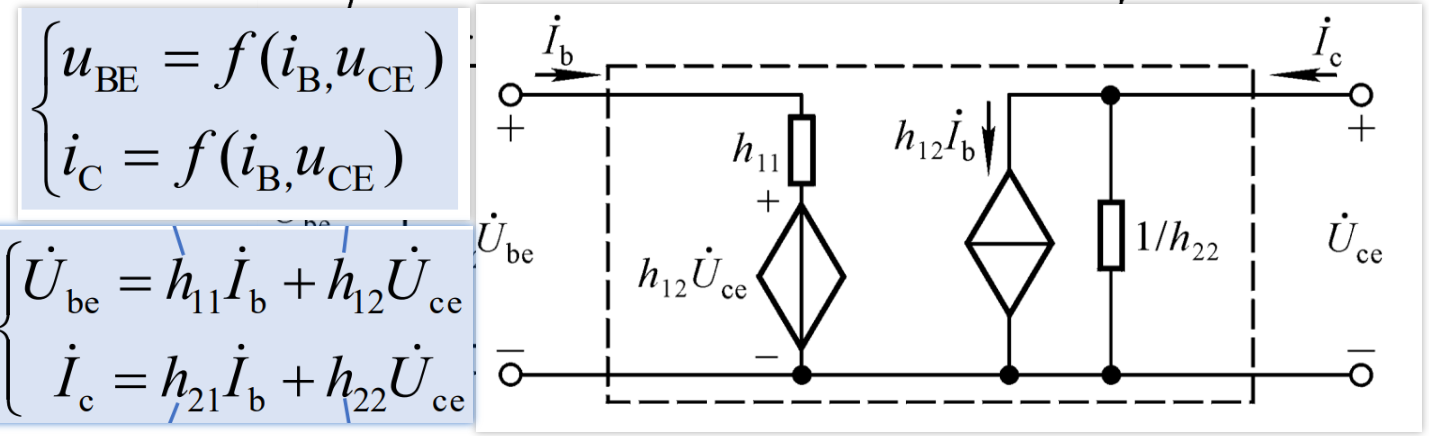
\includegraphics[width=8cm]{img/2.9.png}
            \end{figure}
并且一般的来说有如下
\begin{align}
 h_{11}=r_{be}\thickapprox 0\tag{3.3.a} \\
 h_{12}=\frac{\Delta_{BE}}{\Delta_{CE}}\tag{3.3.b} \\
 h_{21}=\beta\thickapprox \infty\tag{3.3.c} \\
 h_{22}=\frac{1}{r_{ce}}\tag{3.3.d} 
\end{align}
继续简化就可以得到
\begin{figure}[H]
    \centering
    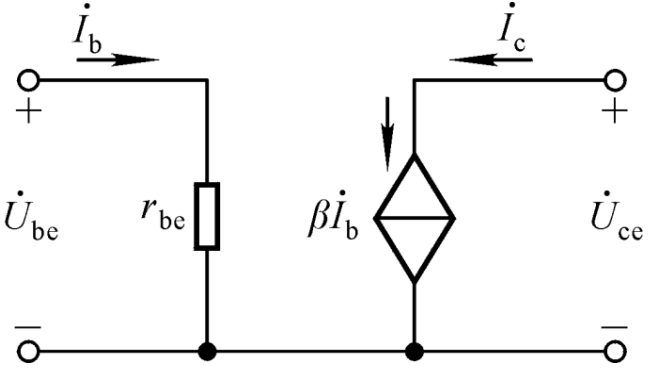
\includegraphics[width=7cm]{img/2.10.png}
    \end{figure}
并且有$r_{bb'}$ 为基区体积电阻,$r_{b'e}$为发射结微分电阻,$r_{ce}$为集电结微分电阻,$U_T=26(mV)$。
\begin{figure}[H]
    \centering
    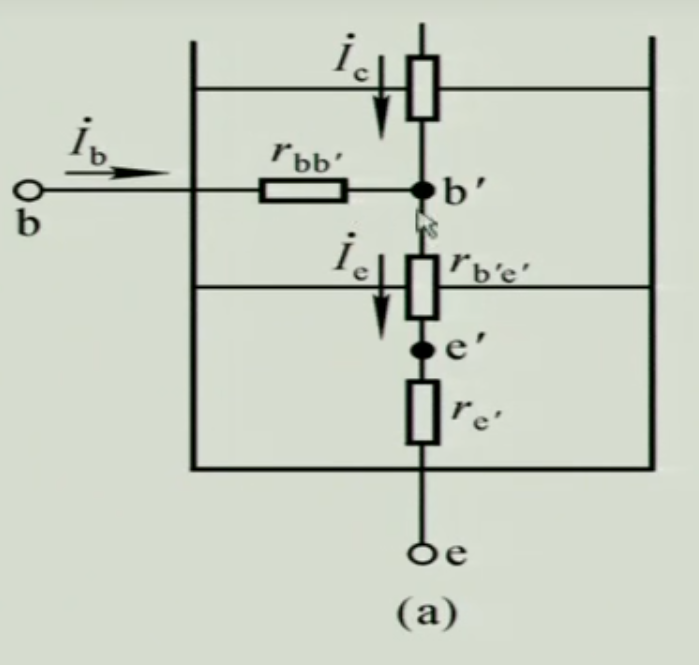
\includegraphics[width=7cm]{img/2.12.png}
    \end{figure}
$$ 
\begin{aligned}
    U_{be}&=I_b(r_{bb'})+I_{e}(r_{b'e}) \\
    r_{be}&=\frac{U_{be}}{I_b}=r_{bb'}+r_{b'e}
    \\&=r_{bb'}+(1+ \beta)\frac{U_T}{I_{EQ}(mA)} 
    \\&=r_{bb'}+\frac{U_{T}}{I_{BQ}}
\end{aligned}
$$
\subsubsection{直接接法}
之前等效的左b右c下e。VCC对交流短路,所以可直接当接地。具体如下图
        \begin{figure}[H]
            \centering
            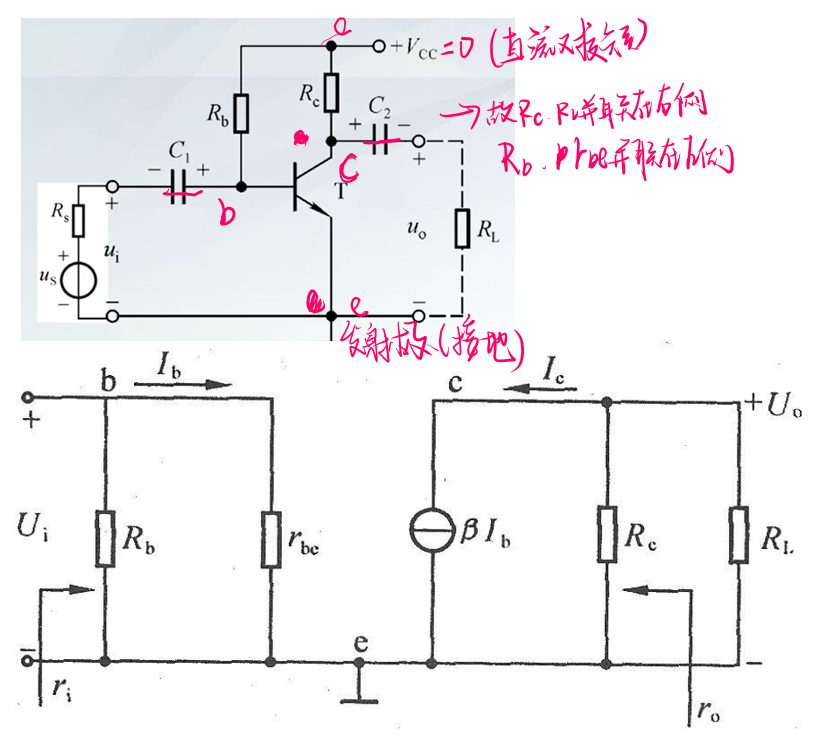
\includegraphics[width=7cm]{img/2.11.png}
            \end{figure}
下面计算一些常用参数
\begin{align}
    A_{u}&= \frac{U_{o}}{U_{i}}= \frac{-i_{c}R_{o}}{i_{b}r_{be}}=- \frac{\beta R_{o}}{r_{be}} \tag{3.4.a} \\
    R_i&=\frac{U_i}{I_i}=R_b // r_{be} \tag{3.4.b}\\
    R_o&=\frac{U_o}{I_o}=R_c // R_L\thickapprox R_c \tag{3.4.c}\\
    r_{be}&=r_{bb'}+\frac{U_T}{I_{BQ}} \tag{3.4.d}\\
    A_I&\thickapprox \beta \frac{R_{L}'}{R_L}
\end{align}
\subsubsection{最大不失真电压}
\subsubsection{失真分析}
\subsection{放大电路Q点的稳定性}
温度,电源波动,元器件老化都会引起Q点波动。会失真,截至失真,饱和失真。
\subsubsection{如何稳定}
所谓Q点稳定,是指$ I_{CQ} $ 和 $ U_{CEQ} $在温度变化时基本不变,
这是靠$ I_{BQ} $的变化得来的(加了反馈电阻$R_e$)。
        \begin{figure}[H]
            \centering
            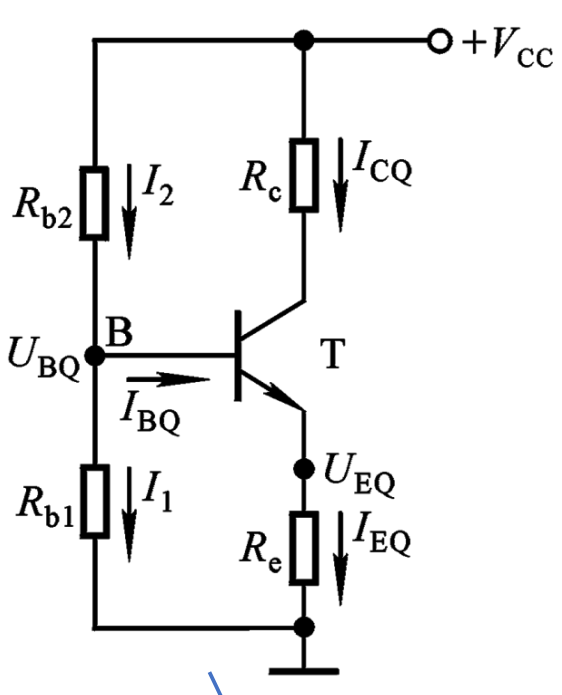
\includegraphics[width=5cm]{img/2.13.png}
            \end{figure}


% \section{第二章}
\subsection{2.2}


\end{document}